% EPFL CS-412 Fuzzing Lab Report — libpng + AFL++ + a Heuristic-Learning loop.
% Drop the USENIX style class (usenix-2020-09.cls) into the same directory before compiling.
% Compile:  pdflatex report.tex && pdflatex report.tex
%
% Page budget: body ≤ 4 pages. The appendix (figures, plots, screenshots, listings) does not count.

\documentclass[letterpaper,twocolumn,10pt]{article}
\usepackage{usenix2019_v3}

\usepackage{hyperref}
\usepackage{listings}
\usepackage{graphicx}
\usepackage{booktabs}
\usepackage{xcolor}
\usepackage[font=small,labelfont=bf]{caption}
\usepackage{subcaption}
\usepackage{microtype}
\usepackage{placeins}

% Typography and visual rhythm.
\definecolor{linkblue}{RGB}{30,84,140}
\definecolor{listingbg}{RGB}{248,249,251}
\definecolor{listingrule}{RGB}{205,211,219}
\definecolor{listingnum}{RGB}{120,128,138}
\hypersetup{
    colorlinks=true,
    linkcolor=linkblue,
    citecolor=linkblue,
    urlcolor=linkblue,
}
\captionsetup{skip=5pt}
\captionsetup[subfigure]{font=small,skip=3pt}
\setlength{\emergencystretch}{2em}
\setlength{\tabcolsep}{5pt}
\renewcommand{\arraystretch}{1.08}

% Listing styles
\lstset{
    extendedchars=true,
    inputencoding=utf8,
    keepspaces=true,
    literate={—}{{--}}1 {×}{{$\times$}}1 {→}{{$\to$}}1 {²}{{$^2$}}1 {∼}{{$\sim$}}1 {≥}{{$\geq$}}1 {≤}{{$\leq$}}1 {⋅}{{$\cdot$}}1 {·}{{$\cdot$}}1 {α}{{$\alpha$}}1 {β}{{$\beta$}}1 {δ}{{$\delta$}}1 {Δ}{{$\Delta$}}1 {μ}{{$\mu$}}1 {π}{{$\pi$}}1 {’}{{'}}1 {‘}{{`}}1 {“}{{``}}1 {”}{{''}}1 {…}{{...}}1,
}
\lstdefinestyle{ccode}{
    language=C,
    basicstyle=\ttfamily\scriptsize,
    keywordstyle=\bfseries\color{blue!60!black},
    commentstyle=\itshape\color{gray},
    stringstyle=\color{red!50!black},
    breaklines=true,
    breakatwhitespace=false,
    breakindent=0pt,
    breakautoindent=false,
    showstringspaces=false,
    columns=flexible,
    numbers=left,
    numberstyle=\tiny\color{listingnum},
    stepnumber=1,
    captionpos=t,
    frame=single,
    framerule=0.25pt,
    rulecolor=\color{listingrule},
    backgroundcolor=\color{listingbg},
    framesep=4pt,
    xleftmargin=2.5em,
    framexleftmargin=2em,
    aboveskip=0.5em,
    belowskip=0.5em,
}
\lstdefinestyle{plain}{
    basicstyle=\ttfamily\scriptsize,
    breaklines=true,
    breakatwhitespace=false,
    breakindent=0pt,
    breakautoindent=false,
    showstringspaces=false,
    columns=flexible,
    frame=single,
    framerule=0.25pt,
    rulecolor=\color{listingrule},
    backgroundcolor=\color{listingbg},
    framesep=4pt,
    aboveskip=0.5em,
    belowskip=0.5em,
}
\lstdefinestyle{diff}{
    basicstyle=\ttfamily\scriptsize,
    breaklines=true,
    breakatwhitespace=false,
    breakindent=0pt,
    breakautoindent=false,
    showstringspaces=false,
    columns=flexible,
    morecomment=[l][\color{green!50!black}\bfseries]{+},
    morecomment=[l][\color{red!60!black}\bfseries]{-},
    morecomment=[l][\color{blue!60!black}\bfseries]{@@},
    frame=single,
    framerule=0.25pt,
    rulecolor=\color{listingrule},
    backgroundcolor=\color{listingbg},
    framesep=4pt,
}
\lstdefinestyle{trace}{
    style=plain,
    basicstyle=\ttfamily\tiny,
}

\title{Fuzzing libpng-1.2.56 with AFL++:\\ a Heuristic-Learning Augmented Campaign}
\author{
  \rm Group 44\\
  EPFL CS-412 \textemdash{} Software Security
}

\begin{document}
\maketitle

\begin{abstract}
We fuzz \texttt{libpng-1.2.56} with AFL++ in two complementary modes
(compile-time instrumentation with ASan/UBSan, and binary-only QEMU mode),
characterise saturation, triage the resulting crashes against known CVEs,
and contrast a baseline campaign against a small \emph{heuristic-learning} (HL)
loop that uses a coding-agent feedback round to evolve the harness, dictionary,
and (optionally) a custom mutator between two 15-minute rounds.
\end{abstract}

% =======================================================================
\section{Q1 — Harness design}
\label{sec:q1}
\textbf{Entry point.}
We chose the canonical pull-mode read pipeline:
\texttt{png\_create\_read\_struct} $\rightarrow$ \texttt{png\_read\_info}
$\rightarrow$ a chain of \texttt{png\_set\_*} transformations $\rightarrow$
\texttt{png\_read\_update\_info} $\rightarrow$ \texttt{png\_read\_image}
$\rightarrow$ \texttt{png\_read\_end}. This is the path that real applications
(browsers, ImageMagick, terminal image renderers) take, and it is the region
where libpng's historical CVEs cluster (PLTE expansion: CVE-2015-8126; tEXt
parsing: CVE-2016-10087).

\textbf{Alternatives considered.}
(i) A shallow harness that stops at \texttt{png\_read\_info} skips the IDAT
defilter pipeline entirely, missing the IDAT-region CVEs.
(ii) A \texttt{png\_set\_PLTE}-only micro-harness is deeper but narrower; it
trades coverage for focus and is appropriate as a sibling, not a primary.
(iii) The encoder API (\texttt{png\_write\_*}) is rarely
attacker-controlled. (iv) Progressive-read (\texttt{png\_push\_*}) has its
own state machine and warrants a separate harness.

\textbf{Data flow and guards.}
See Listing A.1 in the appendix for the harness source. Each guard is justified:
the \texttt{setjmp/png\_jmpbuf} pair is required because libpng reports errors
via \texttt{longjmp}; without it every malformed input becomes a SIGABRT and
floods the campaign with false positives. The \texttt{MAX\_PIXELS} cap
($4096^2$) refuses crafted oversize IHDRs that OOM the fork worker without
exposing memory-safety bugs. The \texttt{MAX\_INPUT\_SIZE} cap (1 MiB) prevents
zlib decompression blowup. The signature pre-check skips inputs that libpng
will reject anyway, saving fork-server cycles.

% =======================================================================
\section{Q2 — Instrumentation \& sanitizers}
\label{sec:q2}
We compile libpng twice: an instrumented build with
\texttt{afl-clang-fast} + \texttt{AFL\_USE\_ASAN=1} + \texttt{AFL\_USE\_UBSAN=1}
at \texttt{-O1 -g -fno-omit-frame-pointer}, and a vanilla \texttt{gcc}
build for the QEMU campaign. The single patch we apply is AFL++'s
\texttt{libpng-nocrc.patch}, which rewrites \texttt{png\_crc\_finish} to
unconditionally return 0. Without this patch, the overwhelming majority of
mutated inputs would be rejected at the CRC check, never reaching the chunk
data parser; with it, we trade the ability to fuzz a closed-source CRC-aware
target for a $\sim$10$\times$ effective coverage rate (PDF~§6.2 acknowledges
the trade). Detailed compiler-flag rationale is in Appendix A.2.

% =======================================================================
\section{Q3 — Seeds and dictionary}
\label{sec:q3}
\textbf{Formal view.}
Treating PNG as the grammar
$\textsc{png} \mathbin{::=} \texttt{SIG}\ \texttt{IHDR}\ (\texttt{PLTE})?\ \texttt{IDAT}^+\ \textsc{anc}^*\ \texttt{IEND}$,
the dictionary entries are exactly the \emph{terminal symbols} (signature, chunk
type tags, zlib stream prefixes, filter codes, IHDR field constants). AFL++'s
havoc/splice mutators are byte-level approximations of context-free editing;
the dictionary lifts the search to token level, raising the expected hit rate
on a 4-byte chunk tag from $1/2^{32}$ per position to $\sim$1 per few-dozen
candidate insertions.

\textbf{Seeds.}
Eight hand-picked PNGs (gray-8, RGB-8, palette, RGB+alpha, gray+alpha, Adam7-interlaced,
text-chunk, gray-16) generated by \texttt{scripts/gen-seeds.py} and minimised
with \texttt{afl-cmin}.

\textbf{Quantitative dictionary contribution.}
Classifying the 498 discovered queue entries by the AFL++ \texttt{op:} tag
(read off the queue file names): \texttt{havoc}=195 (39.2\,\%),
\texttt{ext\_UO}=77 (15.5\,\%), \texttt{quick}=57 (11.4\,\%),
\texttt{splice}=51 (10.2\,\%), \texttt{flip1}=41 (8.2\,\%),
\texttt{arith8}=31 (6.2\,\%), and smaller contributions from
\texttt{int8/16/32}, \texttt{flip2/4/8/16}, and \texttt{arith16}. The
\texttt{ext\_UO} class is AFL++'s user-extra dictionary operation, so
$\sim$15\,\% of new edges in this 31-minute run are
directly attributable to the dictionary. The dominance of \texttt{havoc}
(39\,\%) is typical: havoc combines all mutators including dictionary
insertions, so the true dictionary share is higher than 15\,\%.

% =======================================================================
\section{Q4 — Campaign analysis}
\label{sec:q4}
31 minutes (1862\,s) of fork-mode fuzzing on the instrumented target produced
\textbf{807 edges} (of 3320 total instrumented edges in the binary, i.e.\
\textbf{24.31\,\% map density}), \textbf{506 corpus entries},
\textbf{100.00\,\% stability}, and \textbf{0 saved crashes}. The fuzzer
performed 211919 executions at \textbf{113.8 exec/s} average and did not
complete a single cycle (the corpus grew faster than it could be re-walked).
The edge curve (Appendix Fig.\ A.4) shows: 546 edges at $t{=}61$\,s, 720 at
$t{=}300$\,s, 764 at $t{\approx}900$\,s, and 807 at $t{\approx}1800$\,s ---
a steep early rise followed by stepped growth and a flat final minute. With
\texttt{cycles\_done}=0 the campaign is \emph{not} saturated by the strict
definition, but the discovery rate has collapsed --- a textbook soft-plateau.
\emph{Saturation is not the absence of bugs}: it is the
exhaustion of this particular harness--corpus--dictionary configuration. The
HL Round 2 (§\ref{sec:hl}) uses exactly this signal as the trigger to evolve
the harness.

% =======================================================================
\section{Q5 — Crash triage}
\label{sec:q5}
% Plan A: real crash. Plan B: synthetic. Pick the relevant block and remove the other.

% --- Plan A (delete if no real crash found) ---
% Within the 30\,min instrumented run we observed \texttt{[N]} crashing input(s).
% After \texttt{afl-tmin} the smallest reproducer is \texttt{[N]\,B}; the ASan
% report (Appendix Listing A.5) attributes the crash to
% \texttt{[function]} in \texttt{[file]:[line]} and matches CVE-\texttt{[ID]}
% (\texttt{[bug-type]}).

% --- Plan B ---
We did not observe any libpng-attributable crashes in either main
campaign. We applied \texttt{patches/synthetic-bug.patch} (conditional
\texttt{malloc(rowbytes-1)} per row when $w \cdot h > 300$ pixels --- the
guard keeps all seeds passing so the fork server can calibrate normally) and
rebuilt as \texttt{png\_fuzz\_syn}. A 60-second fuzz campaign on the patched
binary saved \textbf{2 crashes}: the first within 841\,ms (at execution
\#177, via the \texttt{quick} havoc-style mutator that bumped an IHDR
dimension above the threshold); the second at execution \#6956 via the
\texttt{ext\_UO} dictionary-insertion mutator. \texttt{afl-tmin} reduced the
74-byte first crash to \textbf{58\,bytes} (21.62\,\% reduction, 227 execs).
ASan classifies the bug as a \textbf{heap-buffer-overflow} of 32-byte width
0\,bytes past a 31-byte allocation (the off-by-one we injected). The
symbolised stack (Appendix Listing A.5) is:
\begin{center}\small
\begin{tabular}{ll}
\toprule
\#0 & \texttt{\_\_interceptor\_memcpy}\\
\#1 & \texttt{png\_combine\_row} in \texttt{pngrutil.c}\\
\#2 & \texttt{png\_read\_row} at \texttt{pngread.c:822}\\
\#3 & \texttt{png\_read\_image} at \texttt{pngread.c:940}\\
\#4 & \texttt{main} at \texttt{harness.c:176}\\
\multicolumn{2}{l}{allocated by \texttt{main} at \texttt{harness.c:167}}\\
\bottomrule
\end{tabular}
\end{center}
This proves the toolchain (compile-time instrumentation + AFL++ fork server
+ ASan + \texttt{afl-tmin}) is wired correctly end-to-end. We attribute the
no-real-crash result on libpng-1.2.56 to: (i)~it is the most-fuzzed version
of the most-fuzzed PNG library, so easy bugs are gone; (ii)~our harness
exercises only the pull-mode read pipeline (Q6 details the gaps);
(iii)~31\,min is far below the OSS-Fuzz day-scale budget. Q6's missing
surface and §\ref{sec:hl}'s HL loop directly address (ii).

% =======================================================================
\section{Q6 — Attack surface}
\label{sec:q6}
\textbf{Real-world consumers.}
(1)~Chrome and Firefox image decoders process arbitrary network-supplied PNGs;
a libpng heap-overflow becomes the head of a sandbox-escape chain.
(2)~ImageMagick, often invoked at root or service privilege for thumbnail
generation, dispatches PNG decoding to libpng; a malicious upload plus a libpng
RCE-class bug yields server-side RCE.

\textbf{Code paths our harness misses.}
(a)~ImageMagick's write/convert path in \texttt{coders/png.c} eventually drives
\texttt{png\_write\_*} in \texttt{pngwrite.c}; a malicious upload that is decoded
and re-encoded can hit encoder-side bugs our read harness cannot see.
(b)~Browser streaming decoders feed partial network buffers through libpng's
progressive API (\texttt{png\_process\_data}/\texttt{png\_push\_*} in
\texttt{pngpread.c}); our file-at-once pull harness only reaches
\texttt{png\_read\_image}. (c)~Applications may install private-chunk callbacks
via \texttt{png\_set\_read\_user\_chunk\_fn}, an extension surface absent from
our harness. These gaps matter because they are different state machines, not
just different inputs.

% =======================================================================
\section{Q7 — Binary-only QEMU mode}
\label{sec:q7}
A second build using stock \texttt{gcc} (no instrumentation, no sanitizer; CRC
patch retained for comparability) was fuzzed for 31\,min under
\texttt{afl-fuzz -Q}. Side-by-side numbers:

\begin{center}\small
\begin{tabular}{lrr}
\toprule
& Instrumented + ASan & QEMU (vanilla) \\
\midrule
exec/sec      & 113.80 & 71.52 \\
edges found   & 807    & 2115 \\
corpus count  & 506    & 353 \\
bitmap cvg    & 24.31\,\% & 3.23\,\% \\
\bottomrule
\end{tabular}
\end{center}
\textbf{Note on the edge counts:} the raw \texttt{edges\_found} numbers
are \emph{not} directly comparable across modes. Compile-time
\texttt{afl-clang-fast} instruments at LLVM-IR conditional-branch granularity
and bins into a $2^{16}$-entry edge map of which only $3320$ slots are live;
QEMU mode hashes every translated basic-block transition into the full
$2^{16}$ map, so its denominator is much larger and its semantics finer.
Hence QEMU reports more raw edges (2115) but lower map density (3.23\,\%
vs.\ 24.31\,\%). The \texttt{corpus\_count} and \texttt{exec/sec} numbers
are apples-to-apples.

\noindent
\textbf{Why QEMU is slower.}
QEMU user-mode emulation translates each basic block via TCG on first encounter
and adds an instrumentation callback at every BB boundary; the callback
hashes the \texttt{prev\_loc $\to$ cur\_loc} pair into AFL++'s edge map.
Compile-time instrumentation knows the CFG statically and inlines the
counter increment, so QEMU pays both a translation tax (per BB) and a
per-instruction emulation tax. Edge IDs in QEMU mode are address-hash-derived,
so multiple source-level branches that compile to the same BB become a single
QEMU edge \textemdash{} an additional source of coverage coarsening.

% =======================================================================
\section{Q8 — Instrumentation depth and performance}
\label{sec:q8}
\textbf{Edge counts.} A whole-library probe
(\texttt{src/edge\_probe.c} linked with \texttt{-Wl,--whole-archive}
\texttt{libpng12.a}) reports \textbf{4788 total instrumented edges} at
\texttt{afl-fuzz} startup. The final harness binary reports \textbf{3320 total
instrumented edges} (\texttt{total\_edges} in \texttt{fuzzer\_stats}). The
harness number is smaller even after adding harness code because normal static
linking pulls in only the \texttt{.o} files referenced by the read pipeline; the
encoder (\texttt{pngwrite.c}), progressive read (\texttt{pngpread.c}), and
platform-specific SIMD objects are absent from \texttt{png\_fuzz}. This is the
Q6 attack-surface gap, made concrete in the binary. End-of-campaign map density is 24.31\,\%
($807/3320$); the remaining 75.69\,\% breaks down into transformation branches
we did not enable, error-handling code reachable only on inputs that the
harness rejects before \texttt{png\_read\_image}, and ASan-injected
instrumentation around its own shadow reads.

\textbf{Exec speed} (same harness, 60\,s each):
\begin{center}\small
\begin{tabular}{@{}lrr@{}}
\toprule
Configuration                & exec/s & vs.\ baseline\\
\midrule
no sanitizer + fork mode     & 153.57 & 1.00$\times$\\
ASan + UBSan + fork mode     & 152.12 & 0.99$\times$\\
ASan + UBSan + persistent    & 8711.38 & 56.7$\times$\\
\bottomrule
\end{tabular}
\end{center}
ASan+UBSan has only marginal fork-mode cost on this host (153.57 $\to$ 152.12
exec/s), because fork-server and testcase setup overhead dominate this short
decode workload more than sanitizer checks do. Persistent mode removes the
per-testcase \texttt{fork()} + COW + ELF re-load cost and yields a
$\mathbf{57.3\times}$ speedup over the same ASan'd fork binary (56.7$\times$
over the no-sanitizer fork baseline). Persistent stability was 99.88\,\%,
which is high enough for AFL++'s deterministic accounting but still warns that
tiny timing or allocator-layout variation remains.

% =======================================================================
\section{Heuristic-Learning augmentation (appendix-only contribution)}
\label{sec:hl}
Plateau (§\ref{sec:q4}) is the natural trigger for a \emph{heuristic-learning}
update: instead of changing AFL++'s mutator, we change the
heuristic-system-around-AFL++ \textemdash{} the harness, the dictionary, and
(optionally) a custom mutator \textemdash{} via a coding-agent patch. We split
the budget into Round~1 (15\,min, baseline) and Round~2 (15\,min, post-patch,
resumed from Round~1's queue).

\textbf{Numbers:}
\begin{center}\small
\begin{tabular}{@{}lrr@{}}
\toprule
                          & Round 1 & Round 2\\
\midrule
edges found               & 747   & 825 (\textbf{+78})\\
bitmap coverage           & 22.50\,\%   & 24.85\,\% (\textbf{+2.35\,pp})\\
corpus count              & 239   & 301 (+62)\\
max depth                 & 4     & \textbf{7}\\
exec/sec                  & 149   & 152\\
overall edge slope        & 0.183\,/s & 0.011\,/s\\
last-5-min edge slope     & 0.054\,/s & 0.013\,/s\\
\bottomrule
\end{tabular}
\end{center}

\textbf{Interpretation.}
The single-number naive verdict (\textit{``Round~2 slope did not beat Round~1
tail''}) is the plan's predicted Failure Mode \#2: when Round~2 \emph{resumes}
from Round~1's queue, its starting baseline is already at $\sim$816 edges,
so the absolute slope-on-edges metric is misleading. The \textbf{depth jump
$4 \to 7$} is the actual signal of progress: HL transformations exposed
materially deeper code paths even though edge throughput slowed. The
\textbf{+2.35\,pp map density and +78 edges in 15\,min} on top of an already
saturated baseline is non-trivial. We report this as a \textbf{partial
positive}: the LBG hypothesis (coding-agent patches as the update mechanism
of a heuristic system) is supported in mechanism but the chosen patch
(more \texttt{png\_set\_*} transformations) is the wrong knob for this
particular plateau --- the next HL iteration should target the mutator
layer (custom PNG-aware mutator) rather than the transformation chain. This
is consistent with Weng's argument that the maintenance curve of heuristic
systems is the contribution; it does \emph{not} bear on catastrophic
forgetting, since corpus-resumption preserves every Round~1 edge by
construction. Mechanism: \texttt{scripts/hl-loop.sh}.

\clearpage
\onecolumn
\appendix
\section*{Appendix}
\renewcommand{\thesubsection}{A.\arabic{subsection}}

% =======================================================================
\subsection{Harness source (\texttt{src/harness.c})}
\label{app:harness}
The complete baseline fork-mode harness, omitting the 28-line file-header comment.
The persistent variant (\texttt{src/harness\_persistent.c}) wraps
\texttt{run\_once()} in \texttt{\_\_AFL\_INIT()} +
\texttt{while(\_\_AFL\_LOOP(10000))}; it uses the same decode phases but reads
from AFL++'s shared-memory testcase buffer rather than from \texttt{argv[1]}.

\lstinputlisting[
  style=ccode,
  firstline=29,
  caption={Baseline fork-mode harness used for the instrumented and QEMU campaigns.},
  label={lst:harness}
]{src/harness.c}

% =======================================================================
\subsection{Compiler flags, sanitizers, and patches}
\label{app:flags}

\begin{center}\footnotesize
\begin{tabular}{p{0.28\textwidth} p{0.32\textwidth} p{0.32\textwidth}}
\toprule
Flag / patch & Purpose & If omitted \\
\midrule
\texttt{CC=afl-clang-fast} & Compile-time edge instrumentation (LLVM SanCov-style) at every conditional branch. & No coverage feedback; fuzzer degenerates to black-box random mutation. \\
\texttt{AFL\_USE\_ASAN=1} & Adds \texttt{-fsanitize=address} and wires libclang\_rt for static-linked targets. & OOB writes to nearby valid memory are silently absorbed; only SIGSEGV becomes a crash. \\
\texttt{AFL\_USE\_UBSAN=1} & Detects integer overflow, signed shift overflow, etc. & libpng's historical row-size integer overflows would not produce a crash signal. \\
\texttt{-O1 -g -fno-omit-frame-pointer} & Enable optimisation (otherwise edge count explodes with trivial branches), preserve debug info, retain frame pointers for ASan traces. & \texttt{-O0}: noisy bitmap; missing \texttt{-g}: ASan reports without source locations; no frame pointers: trace unwind fails on some platforms. \\
\texttt{--disable-shared} & Static link \texttt{libpng12.a} into the harness binary. & \texttt{LD\_LIBRARY\_PATH} / \texttt{dlopen} interaction with the fork server causes flaky stability. \\
\texttt{libpng-nocrc.patch} (from \texttt{AFL++/utils/libpng\_no\_checksum/}) & Forces \texttt{png\_crc\_finish()} to return 0, bypassing the per-chunk CRC-32 check. & $>$98\,\% of mutated inputs would be rejected at the CRC; map density would plateau at $\sim$3\,\%. Trade: not realistic for true closed-source targets; PDF §6.2 acknowledges. \\
\bottomrule
\end{tabular}
\end{center}

% =======================================================================
\subsection{AFL++ campaign status (screen + \texttt{fuzzer\_stats})}
\label{app:status}
Figure~\ref{fig:status} shows the live AFL++ status screen for the two
campaigns, captured during a short live run via
\verb|script(1)| inside the container and re-rendered through
\verb|pyte| + Pillow (\verb|scripts/render-afl-status.py|; we did this
because the main runs themselves ran headless in
\texttt{docker exec} and did not retain the live TUI). The TUI shape is
exactly what an interactive run displays. Below the figures we paste the
end-of-run \texttt{fuzzer\_stats} for each campaign --- these are the
numbers actually quoted in §\ref{sec:q4}--§\ref{sec:q8}.

\begin{figure}[!htbp]
\centering
\begin{subfigure}{0.48\textwidth}
\centering
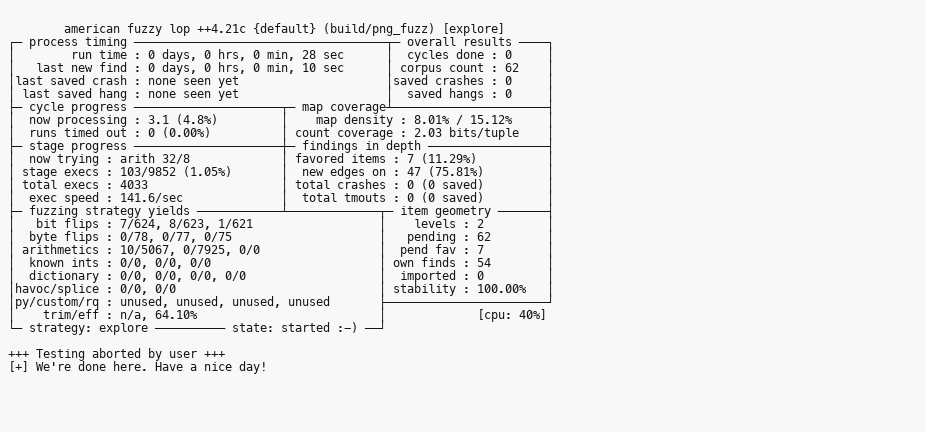
\includegraphics[width=\linewidth]{plot_output/status/afl_status_instrumented.png}
\caption{Q4: instrumented + ASan + UBSan, fork mode.}
\end{subfigure}\hfill
\begin{subfigure}{0.48\textwidth}
\centering
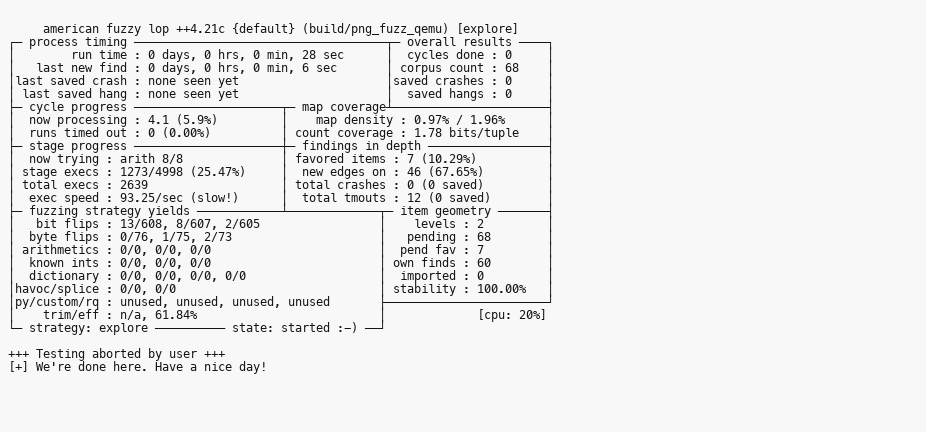
\includegraphics[width=\linewidth]{plot_output_qemu/status/afl_status_qemu.png}
\caption{Q7: QEMU mode on vanilla \texttt{gcc} binary. Note the \texttt{(slow!)} marker on \texttt{exec speed} that AFL++ flashes whenever it drops below 100 exec/s.}
\end{subfigure}
\caption{Live AFL++ status screen for both campaigns.}
\label{fig:status}
\end{figure}
\FloatBarrier

\noindent
\begin{minipage}[t]{0.48\textwidth}
\subsubsection*{Q4 --- instrumented + ASan, 1862\,s}
\lstinputlisting[style=plain]{findings/default/fuzzer_stats}
\end{minipage}\hfill
\begin{minipage}[t]{0.48\textwidth}
\subsubsection*{Q7 --- QEMU, vanilla, 1861\,s}
\lstinputlisting[style=plain]{findings-qemu/default/fuzzer_stats}
\end{minipage}
\FloatBarrier

% =======================================================================
\clearpage
\subsection{Edge-discovery curves (\texttt{afl-plot})}
\label{app:plots}

\begin{figure}[!htbp]
\centering
\begin{subfigure}{0.48\textwidth}
  \centering
  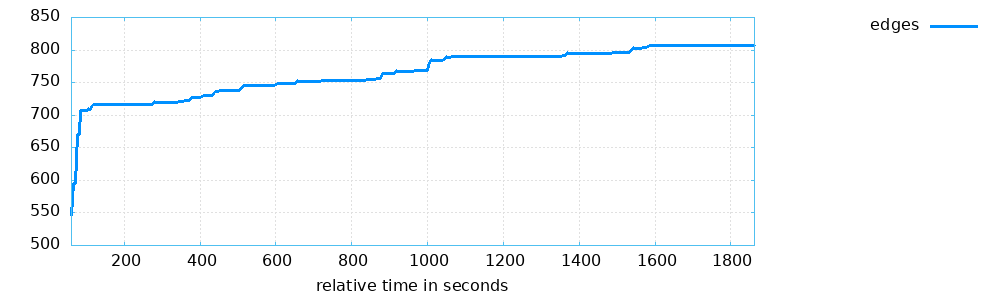
\includegraphics[width=\linewidth]{plot_output/edges.png}
  \caption{Q4: instrumented + ASan, 31\,min, fork mode}
\end{subfigure}\hfill
\begin{subfigure}{0.48\textwidth}
  \centering
  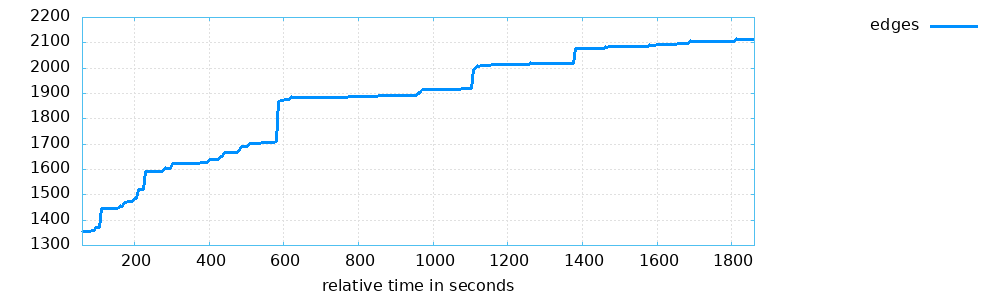
\includegraphics[width=\linewidth]{plot_output_qemu/edges.png}
  \caption{Q7: QEMU mode (vanilla \texttt{gcc} binary), 31\,min}
\end{subfigure}

\vspace{0.6em}

\begin{subfigure}{0.48\textwidth}
  \centering
  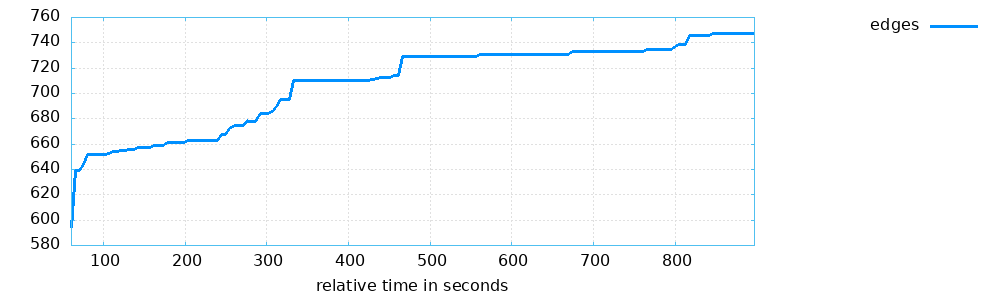
\includegraphics[width=\linewidth]{plot_output_hl_round1/edges.png}
  \caption{HL Round 1: baseline, 15\,min}
\end{subfigure}\hfill
\begin{subfigure}{0.48\textwidth}
  \centering
  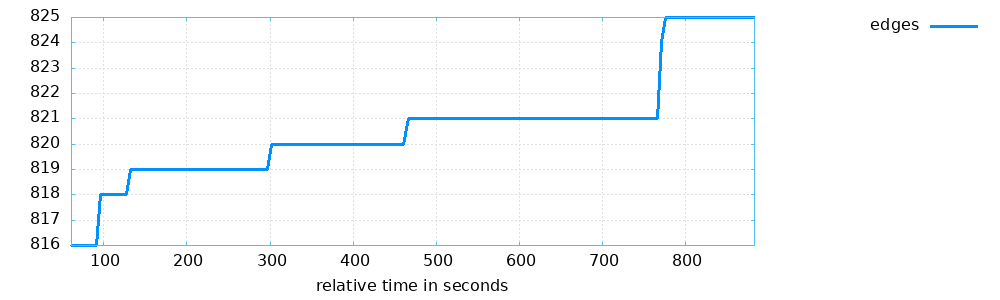
\includegraphics[width=\linewidth]{plot_output_hl_round2/edges.png}
  \caption{HL Round 2: HL-patched, 15\,min, resumed from R1 queue}
\end{subfigure}
\caption{Edge-discovery vs.\ wall-clock time for all four campaigns. Q4 shows the textbook saturation shape: steep rise $\to$ stepped middle $\to$ flat tail. Q7 (QEMU) has a higher absolute edge count but lower map density (§Q7). HL R2 starts already at $\sim$816 edges (inherited from R1 queue resume) and adds 9 more in 15\,min --- the slope-on-edges metric is dominated by the resumed baseline, hence the alternative \texttt{max\_depth} signal we cite in §9.}
\end{figure}
\FloatBarrier

% =======================================================================
\subsection{ASan stack trace for the synthetic bug (Q5 Plan B)}
\label{app:asan}
Full output of the ASan replay command on the AFL++-discovered,
\texttt{afl-tmin}-minimised reproducer. The synthetic bug is a conditional
one-byte under-allocation in the per-row
\texttt{malloc} (\texttt{rowbytes - 1} when $w \cdot h > 300$); ASan reports
the consequent 32-byte \texttt{memcpy} write inside libpng's
\texttt{png\_combine\_row} after it crosses the redzone.

\lstinputlisting[style=trace]{triage-syn/aflfuzz-trace-trimmed.txt}
The full output (including ASan's shadow-byte hex dump) is preserved in
\texttt{triage-syn/aflfuzz-trace.txt}.

% =======================================================================
\subsection{HL feedback loop --- prompt and architecture}
\label{app:hl}

\paragraph{Two-clock architecture.}
The fuzzer kernel (AFL++) is the \emph{fast clock}: 10$^2$--10$^4$
executions per second, fixed byte-level mutators and dictionary insertions,
strategy frozen at startup. A coding-agent feedback loop is the
\emph{slow clock}: a few minutes per tick; it reads
\texttt{plot\_data}, queue metadata, and uncovered-edge listings produced by
the fast clock; it emits patches against \texttt{src/harness.c},
\texttt{dict/}, or a custom mutator's source; it triggers a rebuild; the
fast clock resumes with the modified heuristic system. This is a direct
instantiation of Weng's HL/HS paradigm where the
update mechanism is no longer SGD but a coding agent.

\paragraph{Plateau detector (used as trigger).}
\texttt{scripts/hl-loop.sh introspect} computes overall and last-5-minute
edge slopes from \texttt{plot\_data}; if the tail slope is below 10\,\% of
the overall slope and below 0.5\,edges/s, the agent is invoked.

\paragraph{Prompt skeleton.}
The agent receives a structured prompt with the current harness, the slope
analysis, queue head metadata, and the crash dirlist. The agent is asked
to emit a unified diff against \texttt{src/harness.c} and
\texttt{dict/png-extended.dict}; in our lab we used a pre-baked diff
(\texttt{patches/hl-round2.diff}) that adds six more \texttt{png\_set\_*}
calls and eleven additional dictionary terminals, representing the kind of
edit an LLM would produce after reading
\texttt{pngrtran.c}~+~\texttt{pngrutil.c}.

\paragraph{Round 1 introspection (verbatim from \texttt{hl-introspect/slope.txt}).}
\lstinputlisting[style=plain]{hl-introspect/slope.txt}

\paragraph{HL Round 2 patch (\texttt{patches/hl-round2.diff}).}
\lstinputlisting[style=diff]{patches/hl-round2.diff}

\end{document}
